\documentclass[14pt]{beamer}
%\documentclass[14pt,xcolor=pst]{beamer}

%%%%
%\mode<presentation>
%{
\usetheme{Warsaw}
%}
%\mode<article>
%{
%  \usepackage{fullpage}
%  \usepackage{pgf}
%  \usepackage{hyperref}
%}



%% No stupid navigational symbols
\setbeamertemplate{navigation symbols}{}
%% No footer!
\defbeamertemplate*{footline}{Null}{}
%%%%

\usepackage{graphicx}
\usepackage{ulem}
\usepackage{pstricks,pst-node,pst-text,pst-3d}
%\usepackage{amsmath}
%\usepackage{color}

\title{oftrace:\\An OpenFlow Debugging and Analysis Tool}
%\author{Rob Sherwood~~~Penelope Brooks}
\author{Rob Sherwood ~~~~~ Yiannis Yiakoumis  }
%\newrgbcolor{purple}{.8 0 .8 }

\institute{Stanford Clean Slate Lab}
%\date{IMC 2006}
%\hypersetup{pdfpagemode=FullScreen}

\newcommand{\subbullet}[1]{\begin{itemize}\item #1\end{itemize}}
\newcommand{\subsubbullet}[1]{\begin{itemize}\item #1\end{itemize}}


\begin{document}
%\newlength{\textwidth}
%\setlength{\textwidth}{\textwidth}
\maketitle

%%%%%%%%%%%%%%%%%%%%%%%%%%%%%%%%%%%%%%%%%%%%%%%%%%%%%%%%%%%%%%%%%%%
\begin{frame}
\frametitle{Problem 1/2: Wireshark Hurts My Brain}
\begin{center}
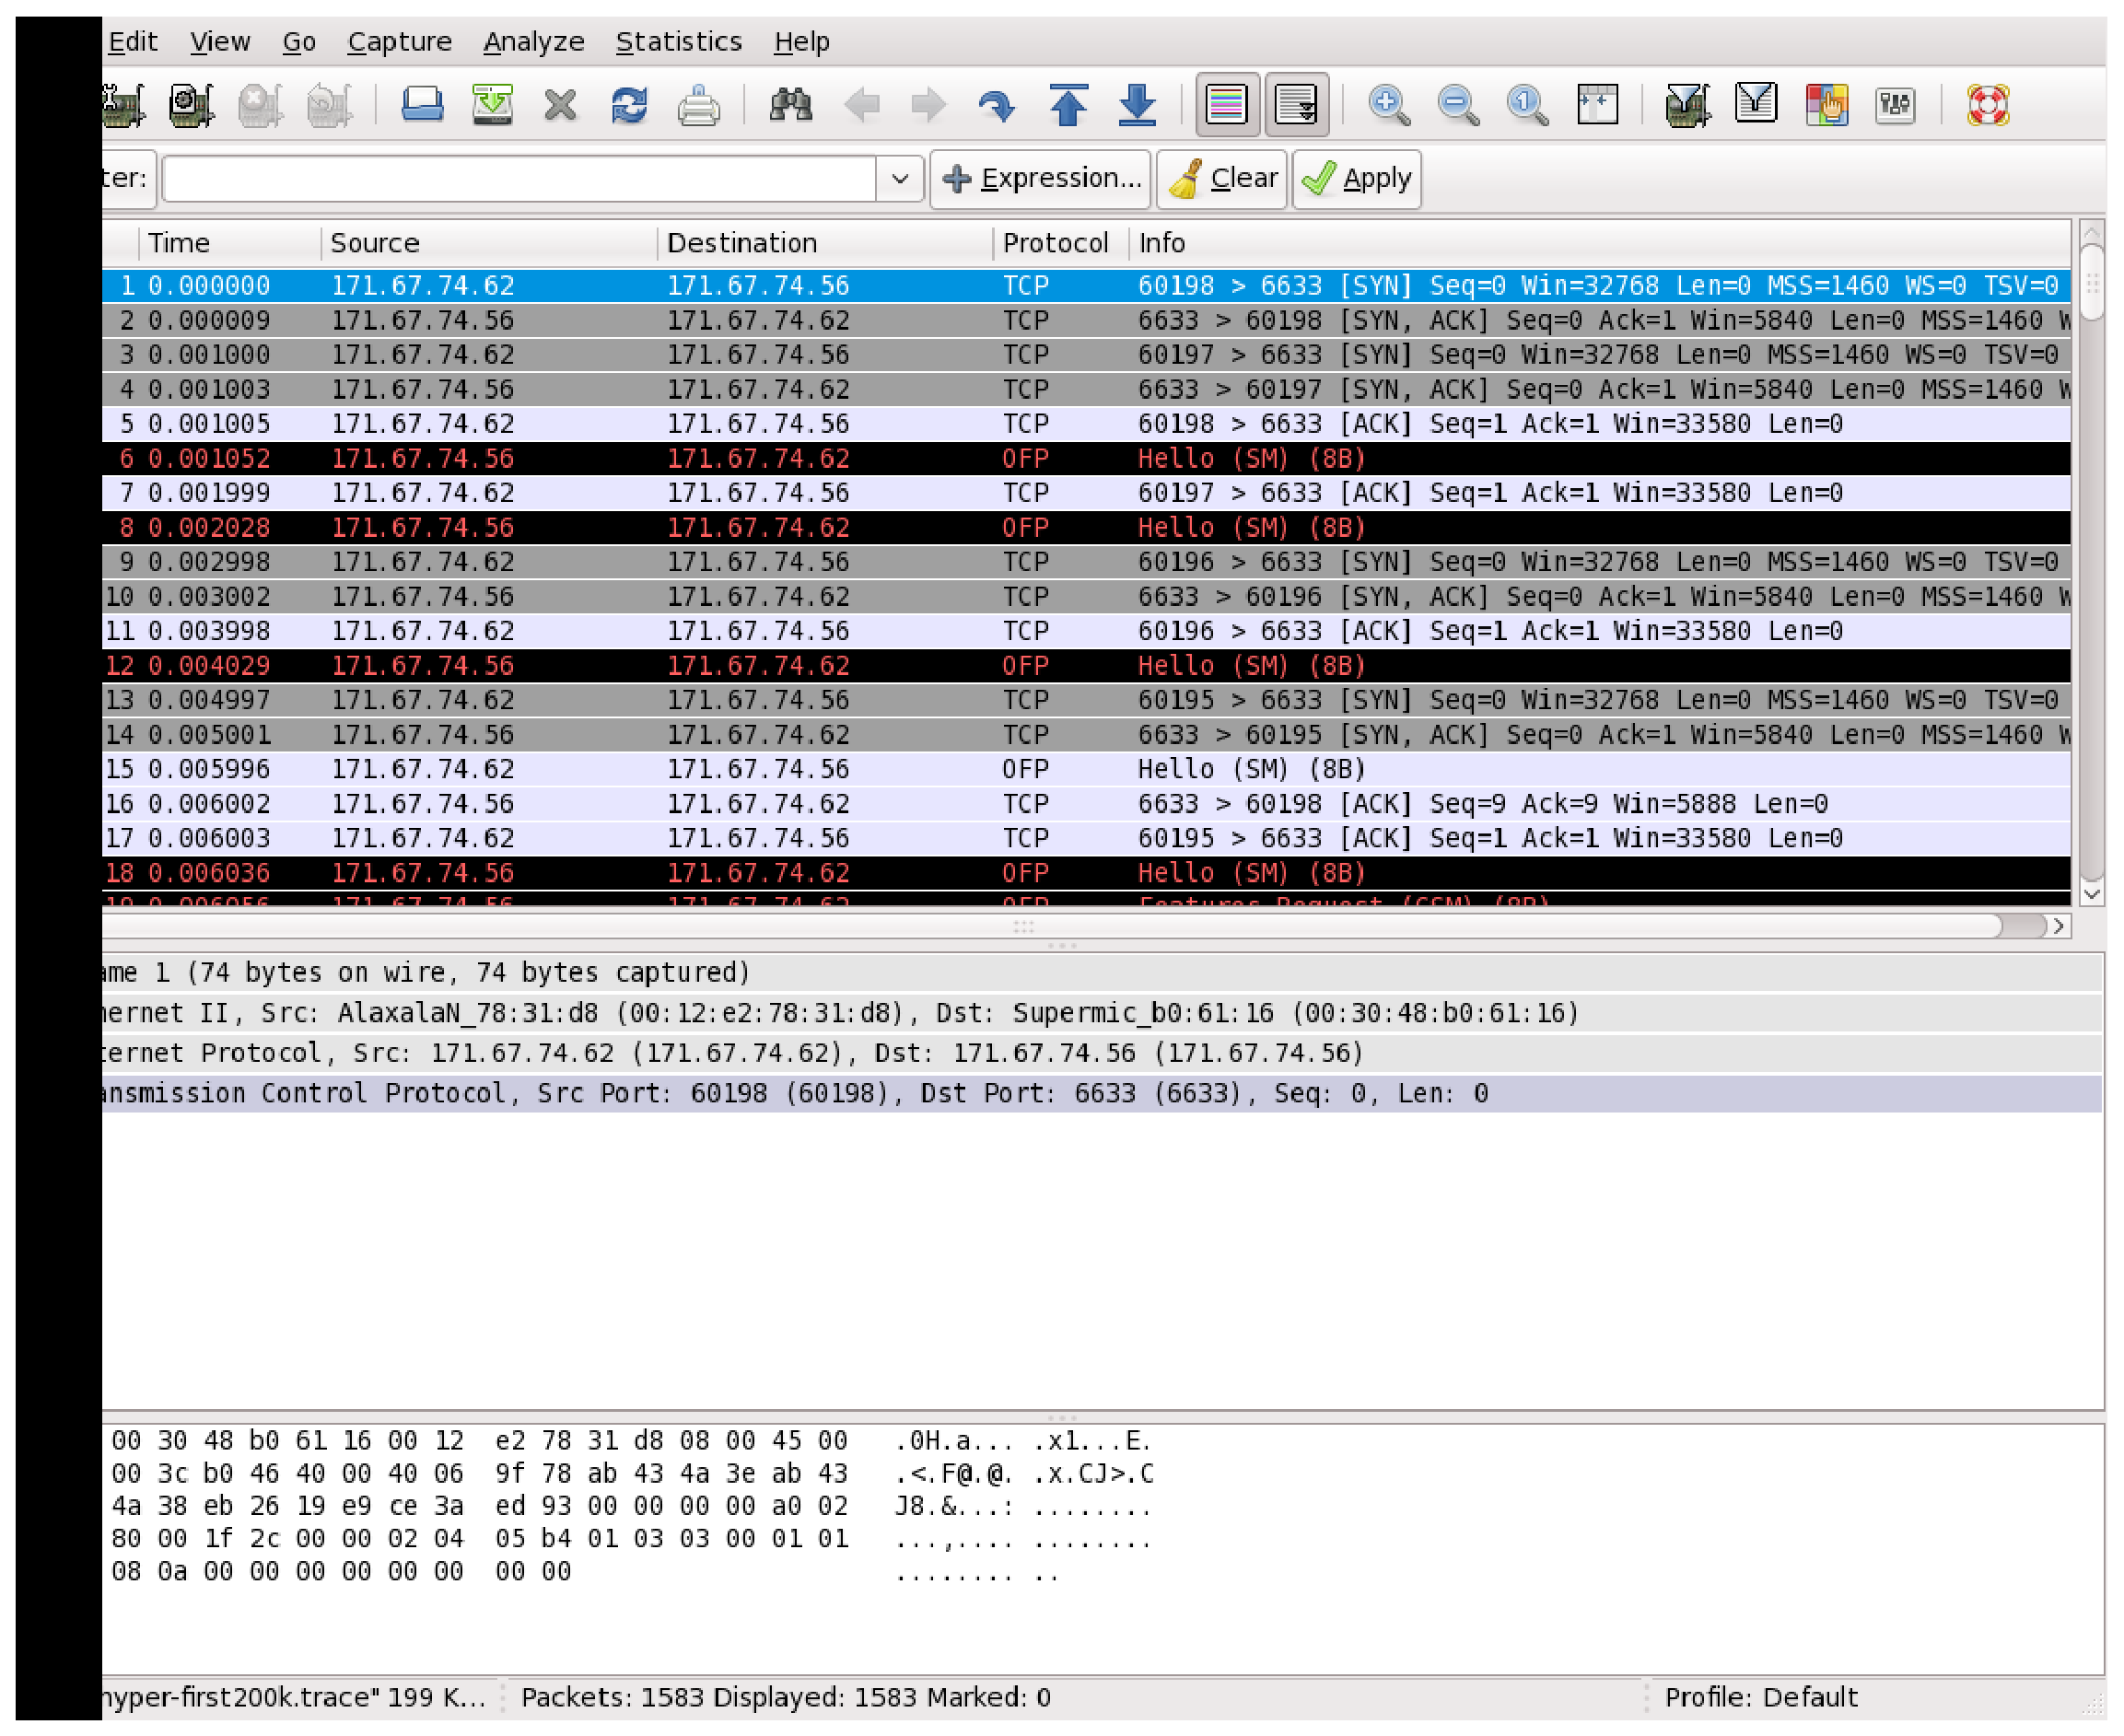
\includegraphics[height=.90\textheight]{figures/wireshark}
\end{center}
\end{frame}
%%%%%%%%%%%%%%%%%%%%%%%%%%%%%%%%%%%%%%%%%%%%%%%%%%%%%%%%%%%%%%%%%%%
\begin{frame}
\frametitle{Problem 2/2: Too Much Data }
\begin{itemize}
\item Apply logical sanity checks
\subbullet{how often do switches send bogus packet? }
\item Calculate aggregate statistics
\item Correlate relations between packet types
\begin{itemize}
\item what is NoX's processing time?
\item how do LLDP packets take?
\end{itemize}
\end{itemize}
\end{frame}
%%%%%%%%%%%%%%%%%%%%%%%%%%%%%%%%%%%%%%%%%%%%%%%%%%%%%%%%%%%%%%%%%%%
\begin{frame}
\frametitle{Answer: Nox Processing Time}
\begin{center}
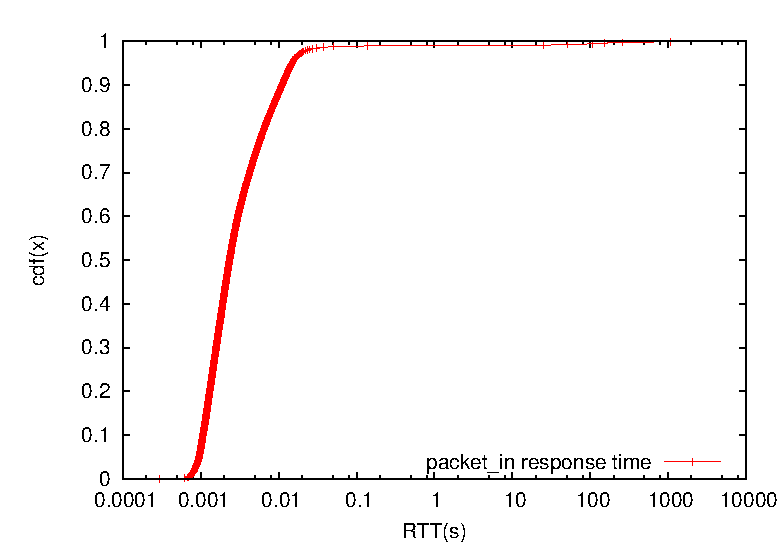
\includegraphics[width=\textwidth]{figures/ofstats_mixed}
\end{center}
\end{frame}
%%%%%%%%%%%%%%%%%%%%%%%%%%%%%%%%%%%%%%%%%%%%%%%%%%%%%%%%%%%%%%%%%%%
\begin{frame}
\frametitle{Answer: LLDP RTT Distribution}
\begin{center}
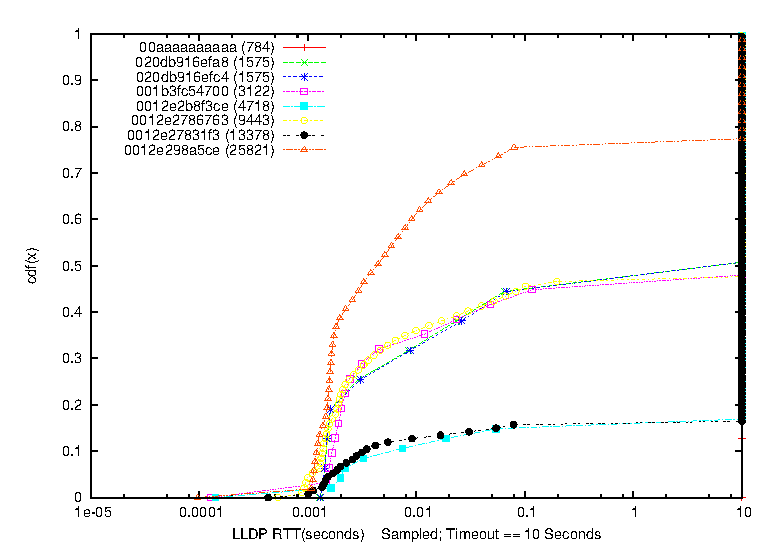
\includegraphics[width=\textwidth]{figures/lldp_by_switch}
\end{center}
\end{frame}
%%%%%%%%%%%%%%%%%%%%%%%%%%%%%%%%%%%%%%%%%%%%%%%%%%%%%%%%%%%%%%%%%%%
\begin{frame}
\frametitle{What Magic Is This? oftrace!}
\begin{itemize}
\item libpcap parsing library
\item Write programmatic queries 
\item Undoes/fixes packet reordering, duplication
\item Simple 4 call API
\item SWIG front end
\subbullet{use your favorite language - not mine}
\end{itemize}
\end{frame}
%%%%%%%%%%%%%%%%%%%%%%%%%%%%%%%%%%%%%%%%%%%%%%%%%%%%%%%%%%%%%%%%%%%
\begin{frame}
\frametitle{Design}
\begin{itemize}
\item Measure everything, all of the time
\subbullet{I always forget to measure {\red something}}
\item No quantum effects
\item libpcap has better timestamps
\item Works for all controllers
\end{itemize}
\end{frame}
%%%%%%%%%%%%%%%%%%%%%%%%%%%%%%%%%%%%%%%%%%%%%%%%%%%%%%%%%%%%%%%%%%%
\begin{frame}
\frametitle{API}
\begin{enumerate}
\item oftrace * {\blue oftrace\_open}(char * pcapfile);
\item const openflow\_msg * {\blue oftrace\_next\_msg}(oftrace * oft, uint32\_t ip, int port);
\item int {\blue oftrace\_rewind}(oftrace * oft);
\item double {\blue oftrace\_progress}(oftrace *oft);
\end{enumerate}
\end{frame}
%%%%%%%%%%%%%%%%%%%%%%%%%%%%%%%%%%%%%%%%%%%%%%%%%%%%%%%%%%%%%%%%%%%
\begin{frame}
\frametitle{Oftrace Mesg Struct}
Raw Data + Convenience Pointers
\begin{enumerate}
\item ethernet header
\item ip header
\item tcp header
\item openflow header
\item (union) openflow message type
\item embedded packets
\item captured size, total size,etc.
\end{enumerate}
\end{frame}
%%%%%%%%%%%%%%%%%%%%%%%%%%%%%%%%%%%%%%%%%%%%%%%%%%%%%%%%%%%%%%%%%%%
\begin{frame}
\frametitle{Example: lldp\_stats.py}
\end{frame}
%%%%%%%%%%%%%%%%%%%%%%%%%%%%%%%%%%%%%%%%%%%%%%%%%%%%%%%%%%%%%%%%%%%
\begin{frame}
\frametitle{Tools}
\begin{itemize}
\item ofdump/pyofdump : lists types and sizes of OF msgs
\item ofstats/pyofstats: controller response time
\subbullet{first graph}
\item lldp\_stats: discovery RTT
\subbullet{second graph}
\item ??
\end{itemize}
\end{frame}
%%%%%%%%%%%%%%%%%%%%%%%%%%%%%%%%%%%%%%%%%%%%%%%%%%%%%%%%%%%%%%%%%%%
\begin{frame}
\frametitle{Implementation}
\begin{itemize}
\item ~700 lines of C (core library)
\item Re-ordering is a pain
\item DLT\_10MB vs. DLT\_LINUX\_SLL
\item Sequence number wrapping 
\item Swig : accessing raw data
\subbullet{cdata}
\end{itemize}
\end{frame}
%%%%%%%%%%%%%%%%%%%%%%%%%%%%%%%%%%%%%%%%%%%%%%%%%%%%%%%%%%%%%%%%%%%
\begin{frame}
\frametitle{TODO}
\begin{itemize}
\item Better filter support
\item Remove PAWS bugs (fixed?)
\item Live capture mode
\end{itemize}
\end{frame}
%%%%%%%%%%%%%%%%%%%%%%%%%%%%%%%%%%%%%%%%%%%%%%%%%%%%%%%%%%%%%%%%%%%
\begin{frame}
\frametitle{Conclusion}
\begin{itemize}
\item Analyzing OpenFlow can be painful
\item oftrace can help you
\item I've written some tools that I think are useful
\item Please contribute your own 
\item http://www.openflowswitch.org/wk/Liboftrace
\end{itemize}
\end{frame}
%%%%%%%%%%%%%%%%%%%%%%%%%%%%%%%%%%%%%%%%%%%%%%%%%%%%%%%%%%%%%%%%%%%
\end{document}

